\pc{1}{31/1}

\question Compute the arrays $d$ and $\pi$ when Dijkstra's algorithm is performed 
on the weighted directed graph $G$ found in Figure \ref{fig:pc-01-1}
(assuming that we start at vertex 1).
\begin{figure}[]
    \centering
    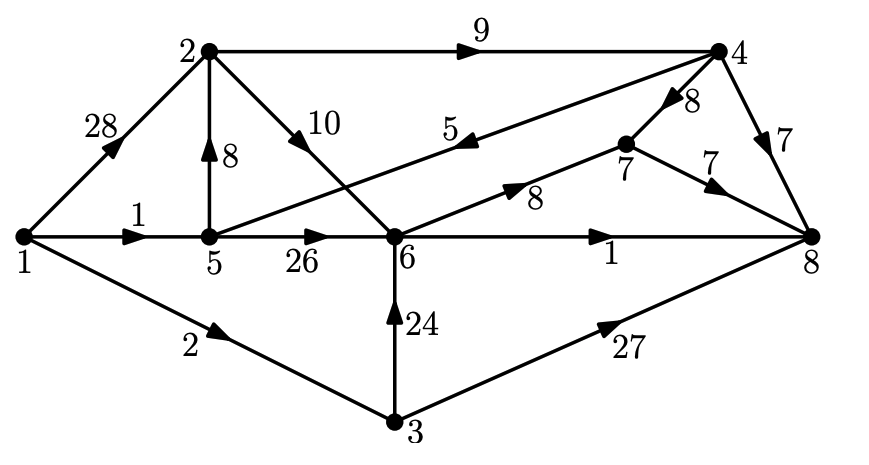
\includegraphics[width=0.8\linewidth]{images/pc-01-1.png}
    \caption{}
    \label{fig:pc-01-1}
\end{figure}
 \begin{solution}
    \begin{center}
        \begin{tabular}{ccc}
            \toprule
            $v$ & $d$ & $\pi$ \\
            \midrule
            1 & - & - \\
            2 & 9 & 5 \\
            3 & 2 & 1 \\
            4 & 18 & 2 \\
            5 & 1 & 1 \\
            6 & 19 & 2 \\
            7 & 26 & 4 \\
            8 & 20 & 6 \\ 
            \bottomrule
        \end{tabular}
    \end{center}
\end{solution}

\question Let $(G, w)$ be an undirected graph without cycles of negative length.
Show that the following algorithm calculates the distances of each vertex
from a given \emph{source} vertex $s$ and determine the time-complexity of the
algorithm.
\begin{algorithm}
    \begin{algorithmic}[1]
        \Procedure{Bellman-Ford}{$G, w, s; d$}
            \State $d(s) \gets 0$
            \For{$v \in V \setminus \{s\}$}
                \State $d(v) \gets \infty$
            \EndFor
            \For{$i = 1$ to $\lvert V \rvert - 1$}
                \For{every edge $uv \in E$}
                    \If{$d(v) > d(u) + w(uv)$}
                        \State $d(v) \gets d(u) + w(uv)$
                    \EndIf
                    \If{$d(u) > d(v) + w(uv)$}
                        \State $d(u) \gets d(v) + w(uv)$
                    \EndIf
                \EndFor
            \EndFor
        \EndProcedure
    \end{algorithmic}
\end{algorithm}

\begin{solution}
    At the $i$th stage of the iteration, we are finding the shortest path between
    the source node and every other node with a maximum of $i$ edges.
    So, as the maximum length of a path between two nodes is $\lvert V \rvert - 1$
    and we have that many iterations,
    the algorithm will find the shortest path between the source and all
    other nodes.
    The Bellman-Ford algorithm has time complexity 
    $O(\lvert V \rvert \lvert E \rvert)$.
\end{solution}

\question Consider the directed network shown in Figure \ref{fig:pc-01-2}, where the edges are marked
with capacities.
Find a maximum flow from $s$ to $t$ and justify your answer.

\begin{figure}[]
    \centering
    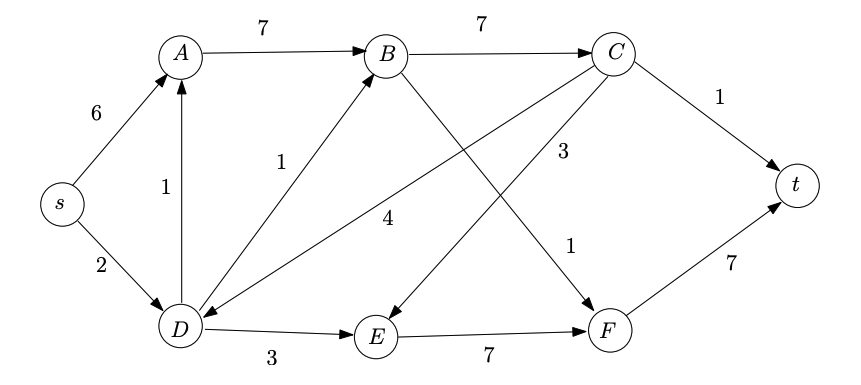
\includegraphics[width=0.8\linewidth]{images/pc-01-2}
    \caption{}
    \label{fig:pc-01-2}
\end{figure}

\begin{solution}
    A maximal flow $8$, shown below.
    \begin{center}
        \begin{tikzpicture}
            \tikzstyle{v}=[circle, minimum size=2em,draw,thick]
            % NODES
            \node[v] (s) {$s$};
            \node[v] (A) [above right= of s] {$A$};
            \node[v] (B) [right= of A]       {$B$};
            \node[v] (C) [right= of B]       {$C$};
            \node[v] (D) [below right= of s] {$D$};
            \node[v] (E) [right= of D]       {$E$};
            \node[v] (F) [right= of E]       {$F$};
            \node[v] (t) [below right= of C] {$t$};
            % EDGES
            \draw[->] (s) to node[above left]  {6} (A);
            \draw[->] (A) to node[above]       {6} (B);
            \draw[->] (B) to node[above]       {5} (C);
            \draw[->] (C) to node[above right] {1} (t);
            \draw[->] (B) to node[above right=-1.7em and 1em] 
                                               {1} (F);
            \draw[->] (C) to node[below right] {1} (D);
            \draw[->] (C) to node[below right=1.6em and -1.2em] 
                                               {3} (E);
            \draw[->] (F) to node[below right] {7} (t);
            \draw[->] (E) to node[below]       {6} (F);
            \draw[->] (D) to node[below]       {3} (E);
            \draw[->] (s) to node[below left]  {2} (D);
        \end{tikzpicture}
    \end{center}
\end{solution}

\question Transform the following variants of the maximum flow problem to the standard
version that of the lecture (e.g. with edge capacities:
\begin{parts}
    \part In addition to the edges, every vertex also has some positive capacity.
    For a feasible flow in the network we must satisfy additionally the following
    constraints:
    \[
        \forall\; v \in V\setminus\{s\}:
        \sum_{u:(u,v)\in E} f(u,v) \leq c(v)
        \qquad\text{and}\qquad
        \sum_{u:(s,u) \in E} f(s,u) \leq c(s)
    \]
    where $c: V \to \N_0$ are the capacities of the vertices.
    \begin{solution}
        For every vertex $v$, we split it into $v_1$ and $v_2$.
        $v_1$ has all the incoming flow capacities of $v$ and
        $v_2$ has all the outgoing flow capacities of $v$.
        Then the capacity of the edge between $v_1$ and $v_2$
        is the capacity of the $v$.
    \end{solution}

    \part There exist several sources and sinks.
    \begin{solution}
        Make a source vertex and connect them to all the
        sources in the graph with capacity $\infty$
        (same idea with sinks).
    \end{solution}

    \part The network is undirected.
    Formalise the maximum flow problem in undirected graphs and transform
    (reduce) this problem to the standard version of the maximum
    flow problem on directed networks.
    \begin{solution}
        Replace every undirected edge with three directed edge.
        So
        \begin{center}
            \begin{tikzpicture}
                \tikzstyle{v}=[circle, minimum size=2em,draw,thick]
                % NODES
                \node[v] (u)              {$u$};
                \node[v] (v) [left= of u] {$v$};
                % EDGES
                \draw[-] (u) to node[above] {$c$} (v);
            \end{tikzpicture}
        \end{center}
        becomes
        \begin{center}
            \begin{tikzpicture}    
                \tikzstyle{v}=[circle, minimum size=2em,draw,thick]
                % NODES
                \node[v] (u) {$u$};
                \node[v] (v) [above right=1em and 2.5em of u] {$v$};
                \node[v] (w) [below right=1em and 2.5em of u] {$w$};
                % EDGES
                \draw[->] (u) to node[above left] {$c$} (v);
                \draw[->] (v) to node[right] {$c$} (w);
                \draw[->] (w) to node[below left] {$c$} (u);
            \end{tikzpicture}
        \end{center}
    \end{solution}
\end{parts}
